\documentclass[slides]{pgnotes}

\title{Ansible Windows}

\begin{document}

\maketitle

\tableofcontents

\section{Scenario}

\begin{center}
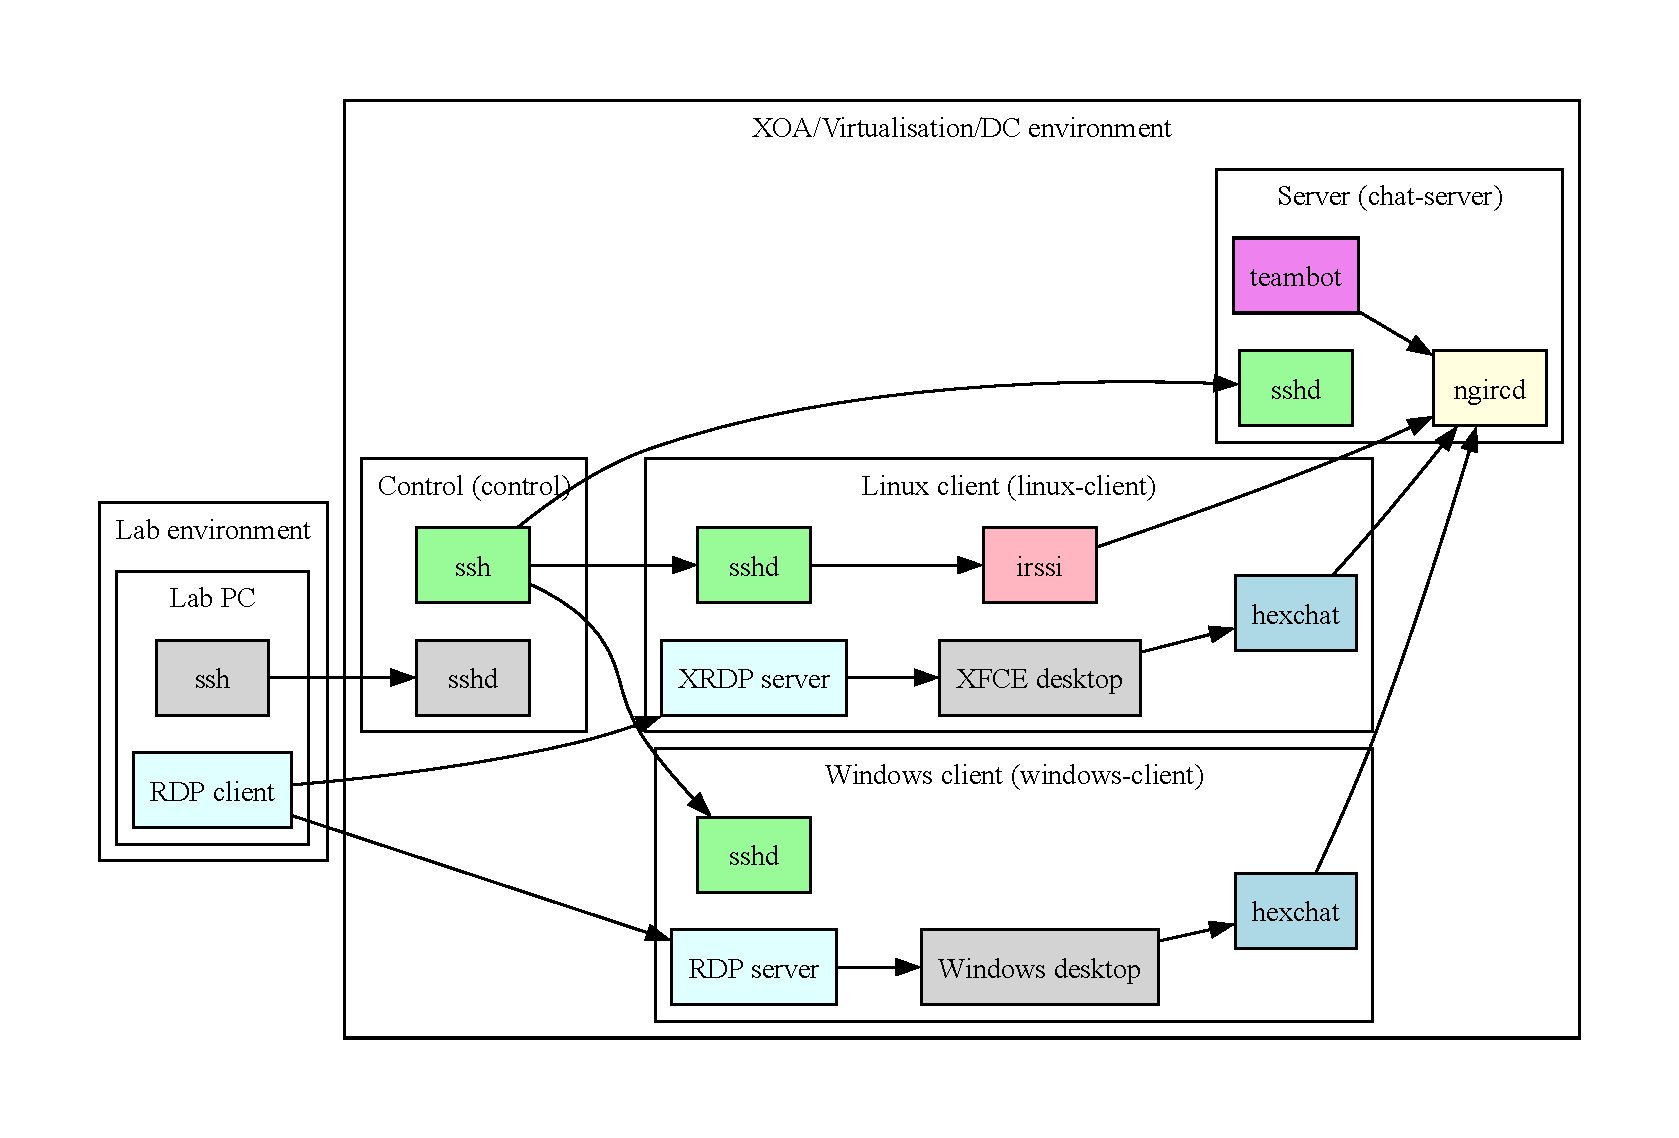
\includegraphics[width=1.0\linewidth]{scenario}
\end{center}


\section{Local ansible usage}

Ansible can be used to automate the machine it's running on (Linux only).

\begin{bluebox}{Sample inventory}
\inputminted{ini}{control_inventory.ini}
\end{bluebox}

\begin{redbox}{Reboots}
  \begin{itemize}
  \item If host reboots then ansible loses its place in the playbook.
  \item Ansible will block reboot instructions in playbooks when running locally.
  \end{itemize}
\end{redbox}

Usage is otherwise the same.


\section{Common use cases}

From ansible guide: 

\begin{enumerate}

\item \textbf{Installing software}

\item \textbf{Installing updates}

\item \textbf{User and group management}

\item \textbf{Command execution}

\item \textbf{File transfer}

\item \textbf{Scheduled task execution}

\item \textbf{Service management}

\end{enumerate}

\section{Complications}

Although Ansible is somewhat \textit{cross-platform} there are some \textbf{specific issues} with Windows:

\begin{enumerate}

\item \textbf{Control node} must be running on \textbf{Linux}.

\begin{itemize}
\item Some experimental support for Windows control nodes but in general it won't work.
\end{itemize}

\item \textbf{Different modules} for same tasks

\begin{itemize}
\item Things like user account creation, hostname setting that in theory are the same on both need different modules on Windows.
\item Playbooks aren't directly portable across Windows / Linux.
\end{itemize}

\item \textbf{WinRM} must be setup at a basic level.

\begin{itemize}
\item Ansible uses WinRM on Windows (rather than SSH) as transport.
\item WinRM can be confusing to setup securely!
\end{itemize}

\end{enumerate}

\end{document}

